Exploring the development and implementation of LessPM, a passwordless password manager, our focus will be on the key
components, technologies, and steps that form the system's development process.
This section will discuss the WebAuthn standard, its effective integration and role in LessPM, and the various security
measures contributing to a robust and reliable solution.

% You should probably blabber some more here but we will do that when we have gotten further with the actual writing.

\newcommand{\credIdentifier}{\footnote{There is a requirement to check whether the credential identifier, generated by the Authenticator
device exsits on the server.
For further discussions on this topic, see section \hyperref[sec:futurework]{Future work}}}

\newcommand{\navigatorApi}{\footnote{In LessPM's case, this is the \textit{navigator.credentials} API provided by the browser.}}

\subsection*{WebAuthn}
WebAuthn, short for Web Authentication, is a collaborative project between the FIDO Alliance and W3C that aims to
implement a secure, robust key-based authentication system for the web, to strongly authenticate users~\cite{webauthn_level_2}.
The concept relies on the use of a third-party device, called an Authenticator, which leverages asymmetric cryptography.
These devices employ biometric or hardware-based mechanisms to provide a secure and reliable means of authenticating a
user.

Upon registration, the Authenticator device generates a key pair called a Passkey.
This Passkey contains a credential ID uniquely generated for each registered key-pair~\cite{webauthn_credential_id,webauthn_public_key_credential}
on the Authenticator.
The unique generation of each key pair offers the advantage of making it much more difficult for trackers to follow a user
\footnote{This is subject to the key-pair alone. A willing party could still track the user through their email or similar.}.
Further, if an attacker gains access to an individual's Passkey, they might compromise one specific service, whereas
a traditional password could potentially compromise multiple services where password reuse occurs\cite{wang2018next}.
\newpage
\subsubsection*{Registration}
In order to register in a WebAuthn authentication system, the user (i.e., client, browser, phone, etc.) issues a registration request to a
WebAuthn implemented server, called a Relying Party (RP), asking to be registered.
The request contains a body with the relevant user identifier (i.e., username, phone number, email, etc.).
The server responds by initiating a registration ceremony and generates a challenge, which is sent to the client.

The client then calls the browser-integrated WebAuthn API, requesting the Authenticator (i.e., phone, hardware Authenticator device, or similar)
to create a new public key credential.
\footnote{The user is prompted to use their Authenticator to prove their presence, which can involve scanning a QR code, providing a fingerprint, or any other modality supported by the device.} During this process, the Authenticator generates a new key-pair (public and private keys). The Authenticator then signs the challenge received from the server with the private key.

The newly created public key, signed challenge, and additional metadata are combined into a public key credential object,
which the client sends back to the server.

The server verifies the authenticity of the signed challenge and the public key credential object.
If successful, the server stores the user's public key and other relevant information (e.g., user identifier, credential ID)
for future authentication.
The process can be seen in figure 1
\begin{figure}[htbp]
    \centering
    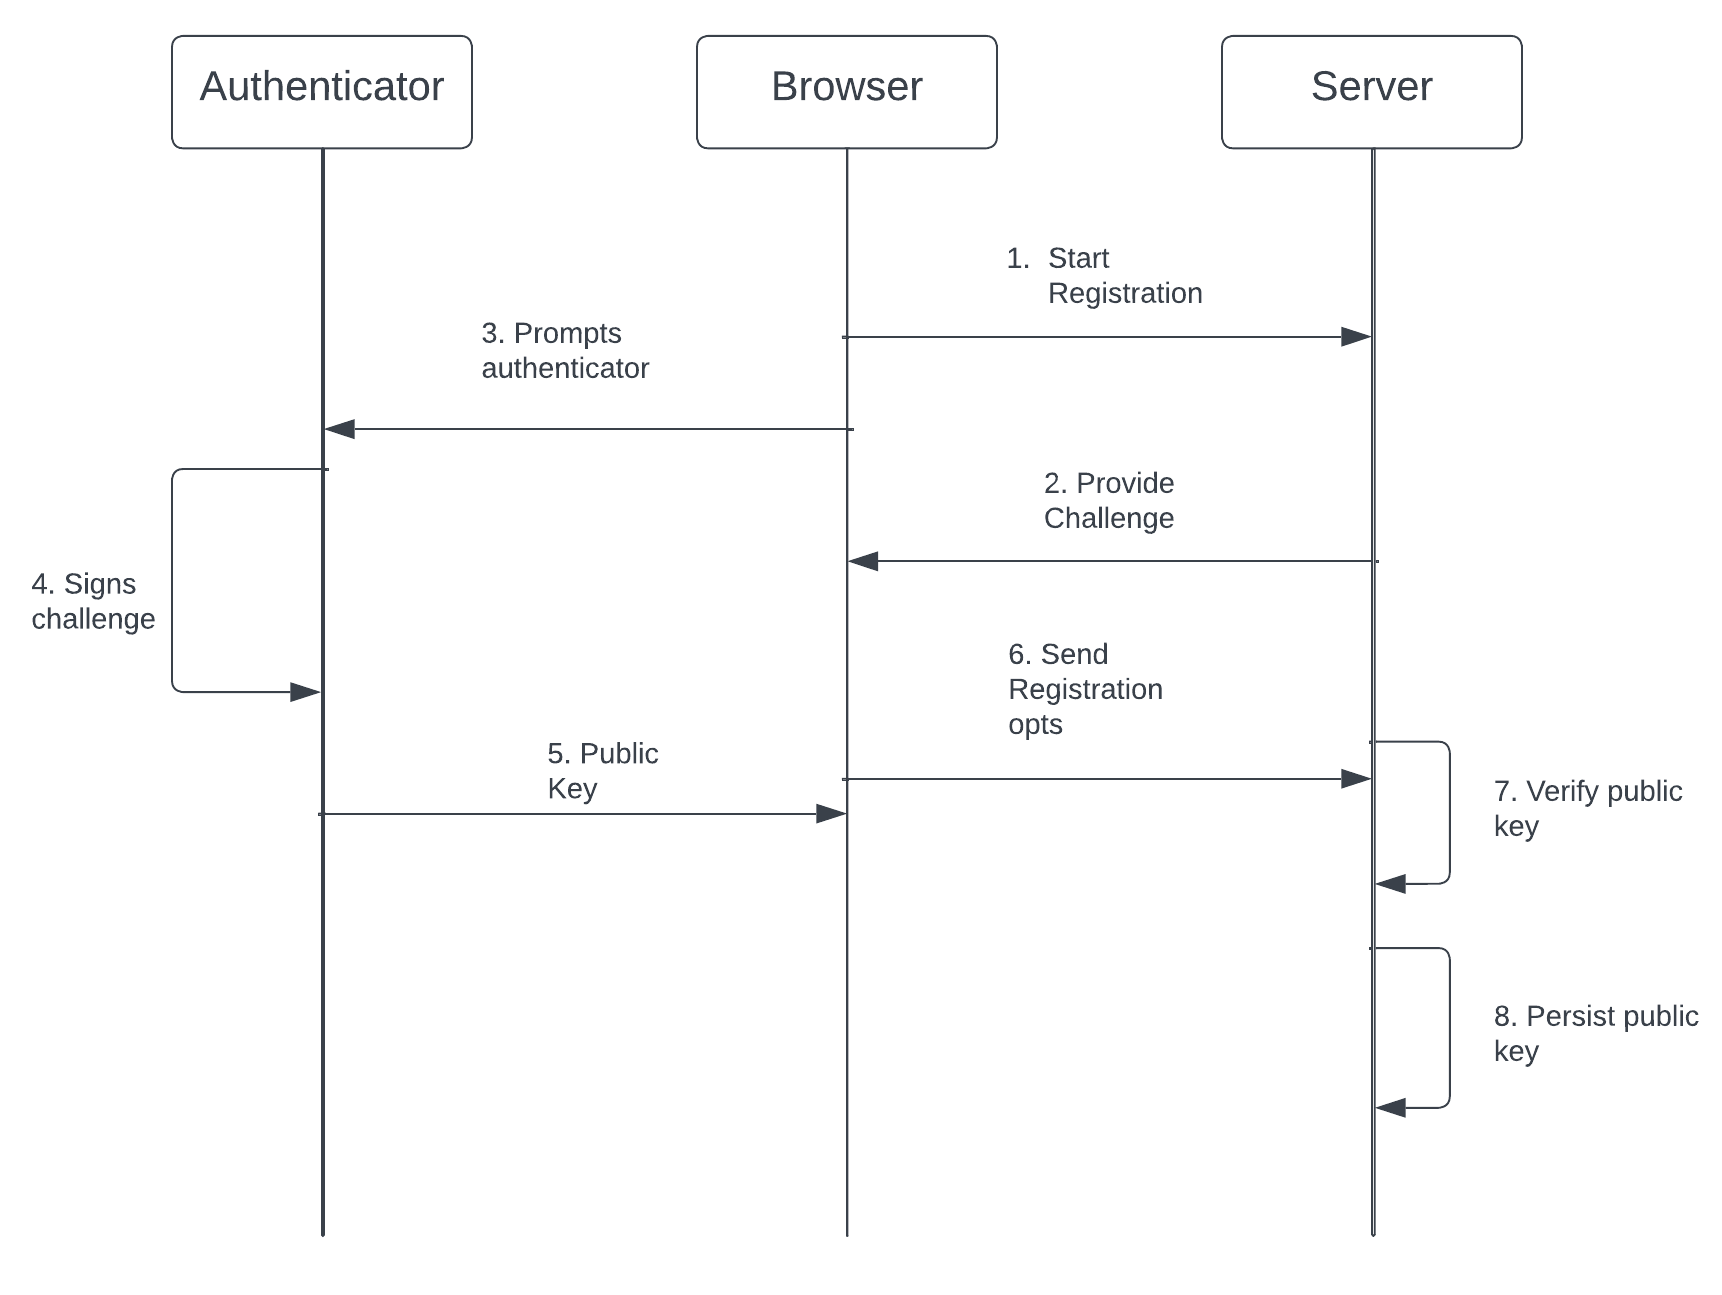
\includegraphics[width=0.85\linewidth]{images/Registration}
    \caption{\footnotesize A diagram dipicting the registration process through WebAuthn and Authenticator Device.}
    \label{fig:your_label}
\end{figure}

\subsubsection*{Authentication}

% Include a diagram

% REGISTRATION
%
%          ┌───────────────┐     ┌───────────────┐      ┌───────────────┐
%          │ Authenticator │     │    Browser    │      │     Site      │
%          └───────────────┘     └───────────────┘      └───────────────┘
%                  │                     │                      │
%                  │                     │     1. Start Reg     │
%                  │                     │─ ─ ─ ─ ─ ─ ─ ─ ─ ─ ─▶│
%                  │                     │                      │
%                  │                     │     2. Challenge     │
%                  │                     │◀ ─ ─ ─ ─ ─ ─ ─ ─ ─ ─ ┤
%                  │                     │                      │
%                  │  3. Select Token    │                      │
%             ─ ─ ─│◀ ─ ─ ─ ─ ─ ─ ─ ─ ─ ─│                      │
%  4. Verify │     │                     │                      │
%                  │  4. Yield PubKey    │                      │
%            └ ─ ─▶│─ ─ ─ ─ ─ ─ ─ ─ ─ ─ ─▶                      │
%                  │                     │                      │
%                  │                     │  5. Send Reg Opts    │
%                  │                     │─ ─ ─ ─ ─ ─ ─ ─ ─ ─ ─▶│─ ─ ─
%                  │                     │                      │     │ 5. Verify
%                  │                     │                      │         PubKey
%                  │                     │                      │◀─ ─ ┘
%                  │                     │                      │─ ─ ─
%                  │                     │                      │     │ 6. Persist
%                  │                     │                      │       Credential
%                  │                     │                      │◀─ ─ ┘
%                  │                     │                      │
%                  │                     │                      │
%

% AUTHENTICATION
% //
% //          ┌───────────────┐     ┌───────────────┐      ┌───────────────┐
% //          │ Authenticator │     │    Browser    │      │     Site      │
% //          └───────────────┘     └───────────────┘      └───────────────┘
% //                  │                     │                      │
% //                  │                     │     1. Start Auth    │
% //                  │                     │─ ─ ─ ─ ─ ─ ─ ─ ─ ─ ─▶│
% //                  │                     │                      │
% //                  │                     │     2. Challenge     │
% //                  │                     │◀ ─ ─ ─ ─ ─ ─ ─ ─ ─ ─ ┤
% //                  │                     │                      │
% //                  │  3. Select Token    │                      │
% //             ─ ─ ─│◀ ─ ─ ─ ─ ─ ─ ─ ─ ─ ─│                      │
% //  4. Verify │     │                     │                      │
% //                  │    4. Yield Sig     │                      │
% //            └ ─ ─▶│─ ─ ─ ─ ─ ─ ─ ─ ─ ─ ─▶                      │
% //                  │                     │    5. Send Auth      │
% //                  │                     │        Opts          │
% //                  │                     │─ ─ ─ ─ ─ ─ ─ ─ ─ ─ ─▶│─ ─ ─
% //                  │                     │                      │     │ 5. Verify
% //                  │                     │                      │          Sig
% //                  │                     │                      │◀─ ─ ┘
% //                  │                     │                      │
% //                  │                     │                      │
%
% using a web server

% Content served over HTTPS through a self-signed certificate
    % Axum as a framework to serve HTTP-content
    % Cors configuration
    % Preflight-mention to the client
    % Allow authorization and cookie
    % cookie stored in HttpOnly (inaccessible to JS). And expiry time which is the same as the JWT.
    % JWT - you only have one minute to login after the request is performed. RSASSA-PSS using SHA-512
    % Find some information about the JWT and use as a reference to talk about the transiton to JWE
    % From JWT -> JWE
    % - For security purposes, there should have been a new key for EACH JWT process
    % There are 15 minutes to interact and do what you want after you're signed in.
    % Password is copiable from the client but does disappear after 15 seconds.
    % The server acts as a one source of truth, client is ONLY rendering and doesn't store anything
    % (other than the cookie)

    % From PBKDF2 (SHA256) to Argon2
    % Argon configuration related to my system
    % Security over usability (In this case)

    % A longer text about WebAuthn, part of the FIDO-2 standard, a validator key that is UNIQUE across all registrations
    % - makes it more difficult to track (suseptiable to email and the likes still).
    % The key is stored in the database with the user

    % Explain the encryption process in detail
    % From generating a 416-bit HASH; 192 from the client validator, 96 from a random padding, 128 from the pepper.

    % First, we generate a "key". This key consists of:
    % - 192 bits from the client validator.
    %   - The validator is different in size, tested on an iPhone 13 pro max, Samsung S21, MacBook Pro 16 inch Intel i9.
    %   - Since the validator is different in size, we stop at 24 byte. If the validator is shorter, we PAD.
    %   - So password A has the validator + a potential, necessary padding to reach 24 byte
    %   - Password B has the validator + a potential, necessary padding to reach 24 byte.
    %   - The padding is unique for each password and each validator.
    % - 96 bits of randomly generated padding.
    % - 128 bits from a pepper.

    % After the key construction, we generate a salt of 96 bit. This salt gets mixed into the Argon2 hash.
    % This constructs the hash, and the hash acts as the key for AES, so it is random.

    % We use this HASH as the key for AES256_GCM to encrypt the data (password) encoding that result in Base64, which is
    % then stored in a database along with:
    % - the username the user selected
    % - the random_padding (that was used to generate the key)
    % - the uuid assigned to the user (used for retrieval)
    % - the nonce (mixed in with AES256)
    % - the key_padding (which is the necessary bits to reach 24 of the validator)
    % - the salt (the one getting mixed in with the hashing

    % The password itself gets encrypted with AES256, where the generated is the hash from the previous step
    % and an appended nonce of 12 byte.

    % A mention to the libraries that are being used, all of them profiled and highly scruitiniced with
    % millions of downloads

    % a proof of concept, that is the client
    % All the client knows is a cookie, which is a JWT, encrypted with RSA512